Pour implanter la version client / monoserveur, nous construisons l'architecture des \iCode{LindaClient}
et \iCode{LindaServer} ci-dessous. La classe \iCode{linda.server.LindaClient} doit être une implantation de
l'interface Linda.

\begin{figure}[H]
    \centering
    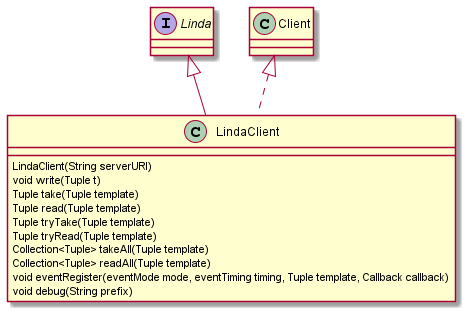
\includegraphics[scale=0.7]{src/part-03/src/fig-4.png}
    \caption{Linda Client} \label{fig:linda-client}
\end{figure}

\iCode{LindaServer} doit être une implantation de l'interface \iCode{LindaRemote} et extension de
\iCode{UnicastRemoteObject}.

\begin{figure}[H]
    \centering
    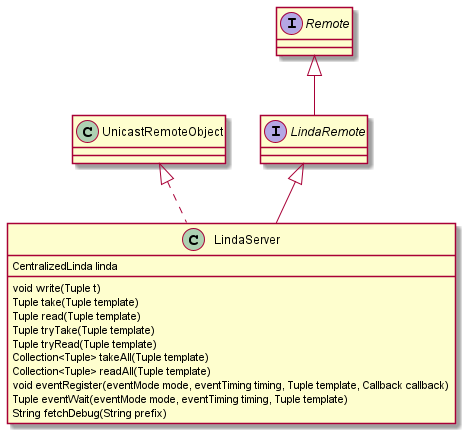
\includegraphics[scale=0.7]{src/part-03/src/fig-5.png}
    \caption{Linda Server} \label{fig:linda-server}
\end{figure}
